\chapter{Implementation}
\label{ch:implementation}
% Prototype level
% geen documentatie manual, maar keuzes en uitdagingen


%\section{Scope}
% Why no iOS?
Due to time constraints we need to focus our implementation effort on a single platform.
Of all mobile devices smart-phones fit our design requirements best.
On smart-phones Android has the largest market share \cite{https://www.statista.com/statistics/266136/global-market-share-held-by-smartphone-operating-systems/}.
We therefore aim our implementation at the largest group of users.

% No routing, no blutooth p2p, mesh networking: that is done by Serval. Out of scope of this work. Add as enhancement later.
We focus on implementing all the features of Tribler as described chapter \ref{ch:tribler} first.
We won't modify the networking capabilities based on the opportunities because that would warrant a dedicated study.


Traditionally applications with a user interface execute tasks in the background while showing the progress to the user.
Due to the fact that Android targets mobile devices it is very optimized for low resource usage.
Therefore memory is freed more aggressively and the application is often paused or stopped and restarted if the user switches to another app.

To run in the background Tribler uses an Android service and all communication is performed asynchronously.
The reactive programming paradigm is a perfect fit for asynchronous tasks.
Thanks to RxJava and RxAndroid asychronous multi-threaded coding is made very enjoyable:
% code example
As shown in the code example performing IO tasks on the dedicated Android thread and making UI changes on the main thread becomes trivial.


memory leak detection


Tribler also uses the event-driven networking engine Twisted, which is written in Python.
API: JSON HTTP server from twisted

API client: retrofit, okhttp


The video player VLC can be integrated as hard to maintain library and a custom GUI.
This was done first, but afterwards we decided to improve maintainability by packaging the entire Android app installation package (.apk).
Which was also much easier to accomplish in hindsight.

The API combined with Java is better for parallelization than the coarse grained locking by the CPython interpreter.
Shared memory threading in Python code is restricted to single-thread performance because of the global interpreter lock (GIL).


The Retrofit library enables a very declarative API client.
% code example?

reactive programming



Android config changes: don't redo work like disc. channels, use fragments like normal android dev.

% Nu teveel schrijven, later filteren



First, what is required to run Tribler on Android?
Tribler is written in Python and uses various libraries written in C and C++.
To use these libraries on a mobile device they need to be compiled for the right embedded-application binary interface (EABI) including all nonstandard dependencies.
Since ARMv7 is currently supported by most Android phones it is the first to be supported by Tribler for now.


% https://kos.gd/posts/5-ways-to-use-python-with-native-code/
Calling C code directly from Python is possible by using the Python ctypes module to load a native dynamic-link library (.so files on Android) or by using the Python/C API of CPython.
This API enables a library to define functions that are written in C to be callable from Python.
These Python bindings are the glue between pure Python and pure C code.
SWIG can generate the boiler plate code for this.
Libtorrent, one of Triblers' main components, uses Boost.Python to provide a standard C++ API on top of the Python/C API.
Kivy uses Cython
% Many parts are written in C using Cython. \cite{kivy.org}
% The major alternative approach promoted by the community is best represented by Cython. Cython is a Python superset designed to be compiled down to CPython C extension modules. One of the features Cython offers (as is possible from any binary extension module) is the ability to explicitly release the GIL around a section of code. By releasing the GIL in this fashion, Cython code can fully exploit all cores on a machine for computationally intensive sections of the code, while retaining all the benefits of Python for other parts of the application. \cite{http://python-notes.curiousefficiency.org/en/latest/python3/multicore_python.html}


Running two interpreters with Python Kivy front-end and Python Tribler back-end would be doubling memory usage for the interpreter itself and require an inter-process protocol as well.
Native Java with XML front-end and Python Tribler back-end brings the user experience seamlessly in line with the native UI.



The Python/C API is actually so powerful it even provides access to the internals of the interpreter to mess with the global interpreter lock (GIL) which could be released during native C calls to improve the multi-threading performance of Tribler crypto.

The Python-for-Android tool-chain provides a way (called recipes) to build these libraries and bindings with the necessary build tools.

P4A uses the Java native interface (JNI), between Java and C/C++ code, to launch the CPython interpreter from a thin Java Android application.
JNI enables to define functions that are written in C to be callable from Java.


Since API level 18 (Android 4.3 codenamed Jelly Bean MR2) loading native libraries dynamically from Python works properly (apparently).
API level 18 also added support for Bluetooth Low Energy (LE), WiFi scan only mode, key store for app-private keys, hardware credential storage and automated UI testing.
All very useful to Tribler.
Earlier versions of Android already supported NDEF Push with NFC and Wi-Fi P2P (since API level 14), and initiate large file transfers over Bluetooth via NFC (since API level 16).
83.7\% of devices on the Google Play Store run Android 4.3 or higher.


python and toolchain aspect

stable with common tools


% Alternatieven QT, P4A, oudere python projecten
What alternatives are there, besides P4A, to run python code on Android?
0. QPython: scripting, cannot build regular .apk
1. QtAndroid, inmiddels alternative, niet gereed toen wij hieraan werkte (juni 2016, qt 5.7 android service)
2. PGS4A: no longer in development
3. SL4A: no longer in development
% Verdedig P4A keuze
Why is P4A chosen?
% Keuze voor P4A door eerder werk en beste match (legacy)
Because this project continued from previous work (legacy code) build on P4A.
% Crosscompilen met python bindings libraries (en dependencies)
Even though the revamp version was build from scratch, it still is the best choice because it not only provides the Python interpreter, it also is a complete tool-chain to cross-compile native libraries with bindings and build a standalone Android app installation package (.apk).


\begin{figure}
	\centering
	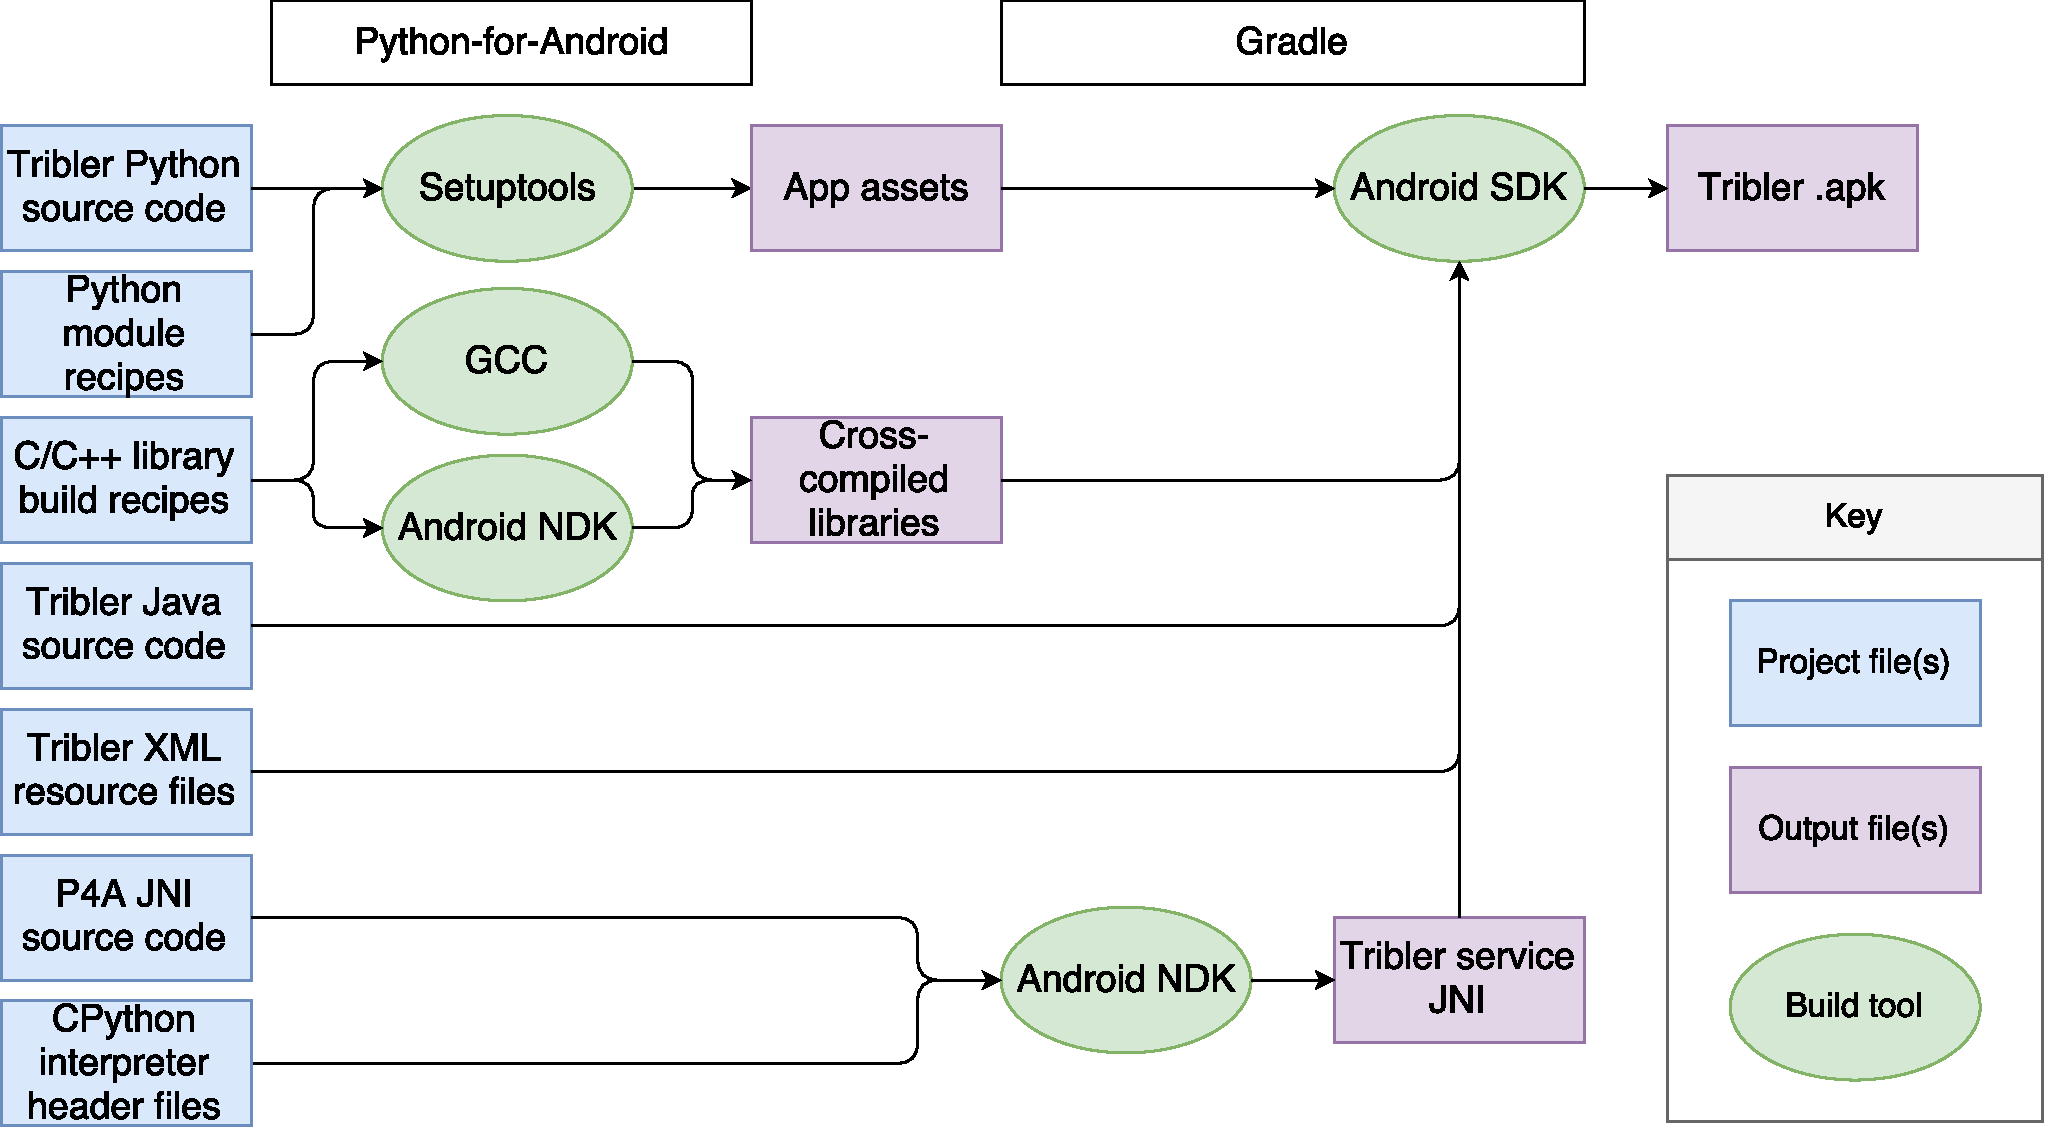
\includegraphics[width=\textwidth]{build_tool_chain}
	\caption{High level overview of the build tool-chain}
	\label{fig:build_tool_chain}
\end{figure}


The Python-for-Android toolchain is used to cross compile the C/C++ libraries (and dependencies) with Python bindings for Android ARMv7.
On top of that the entire core of Tribler can run, containing a REST HTTP API module also written in Python.
The GUI is created by a native Android Java application, which talks to the REST API module.
This Java application contains an Android service that wraps the original P4A CPython launcher.
I changed this behavior to avoid having the GUI and back-end running in the same Python process, hindered by the GIL.
This approach is also superior to having two separate Python interpreters in distinct processes talking to each other, because that means using a very resource heavy Python GUI instead of the regular and lightweight native Android Java XML GUI.
The latter has tools available for automated UI testing.

% ... etc. (@see "my contributions" in thesis)


The Twisted module is used, which uses a single thread to coordinate all others, called the reactor thread.
If this thread is busy, the REST API can not even receive incoming requests resulting in timeouts.
We will investigate this in the next chapter.

Thanks to the design choice of separating the GUI from the back-end this does not result in an unresponsive GUI, like older versions of Tribler are used to.


software stats, delivered, reference github
lang aan gewerkt


The implementation consists of:
12.806 + X lines of code in the Tribler repository in 35 pull requests and
Y lines of code in the Python-for-Android (P4A) repository in 46 pull requests and
2 lines of code in the M2Crypto repository in 1 pull request.
This excludes the work of reviving the old P4A toolchain.

Of the X lines (x \%) consists of unit testing code.
Y lines (y \%) is made up of Android specific libraries, and the remainder is..
Table \ref{table:loc}X shows the 25 largest source file contributions for this thesis work. 

\begin{table}
	\begin{tabular}{l | l | l} \hline
		LOC & File & Path \\ \hline \hline
		718 &		MainActivity.java &		.../org/tribler/android/MainActivity.java \\ \hline
		666 &		MyChannelFragment.java &		.../org/tribler/android/MyChannelFragment.java \\ \hline
		482 &		MyUtils.java &		.../org/tribler/android/MyUtils.java \\ \hline
		403 &		DefaultInteractionListFragment.java &		.../org/tribler/android/DefaultInteractionListFragment.java \\ \hline
		318 &		start.c &		android/TriblerApp/app/src/main/jni/src/start.c \\ \hline
		314 &		TriblerViewAdapter.java &		.../org/tribler/android/TriblerViewAdapter.java \\ \hline
		281 &		build.gradle &		android/TriblerApp/app/build.gradle \\ \hline
		256 &		IRestApi.java &		.../org/tribler/android/restapi/IRestApi.java \\ \hline
		234 &		ChannelFragment.java &		.../org/tribler/android/ChannelFragment.java \\ \hline
		186 &		AssetExtract.java &		.../org/kivy/android/AssetExtract.java \\ \hline
		182 & 		BeamActivity.java &		.../org/tribler/android/BeamActivity.java \\ \hline
		175 &		ListFragment.java &		.../org/tribler/android/ListFragment.java \\ \hline
		172 &		CopyFilesActivity.java &		.../org/tribler/android/CopyFilesActivity.java \\ \hline
		166 &		AndroidManifest.xml &		android/TriblerApp/app/src/main/AndroidManifest.xml \\ \hline
		166 &		EventStreamCallback.java &		.../org/tribler/android/restapi/EventStreamCallback.java \\ \hline
		155 &		ChannelActivity.java &		.../org/tribler/android/ChannelActivity.java \\ \hline
		150 &		ViewFragment.java &		.../org/tribler/android/ViewFragment.java \\ \hline
		149 &		PythonService.java & 		.../org/kivy/android/PythonService.java \\ \hline
		149 &		SearchActivity.java &		.../org/tribler/android/SearchActivity.java \\ \hline
		141 &		EditChannelActivity.java &		.../org/tribler/android/EditChannelActivity.java \\ \hline
		131 &		FilterableRecyclerViewAdapter.java &		.../org/tribler/android/FilterableRecyclerViewAdapter.java \\ \hline
		130 & 		BaseActivity.java &		.../org/tribler/android/BaseActivity.java \\ \hline
		114 &		SearchFragment.java &		.../org/tribler/android/SearchFragment.java \\ \hline
		112 & 		TriblerDownload.java &		.../org/tribler/android/restapi/json/TriblerDownload.java \\ \hline
	\end{tabular}
	\caption{Top 25 of largest source file contributions.}
	\label{table:loc}
\end{table}

Code coverage and testing details are further explained in chapter \ref{ch:results}.


\begin{figure}
	\centering
	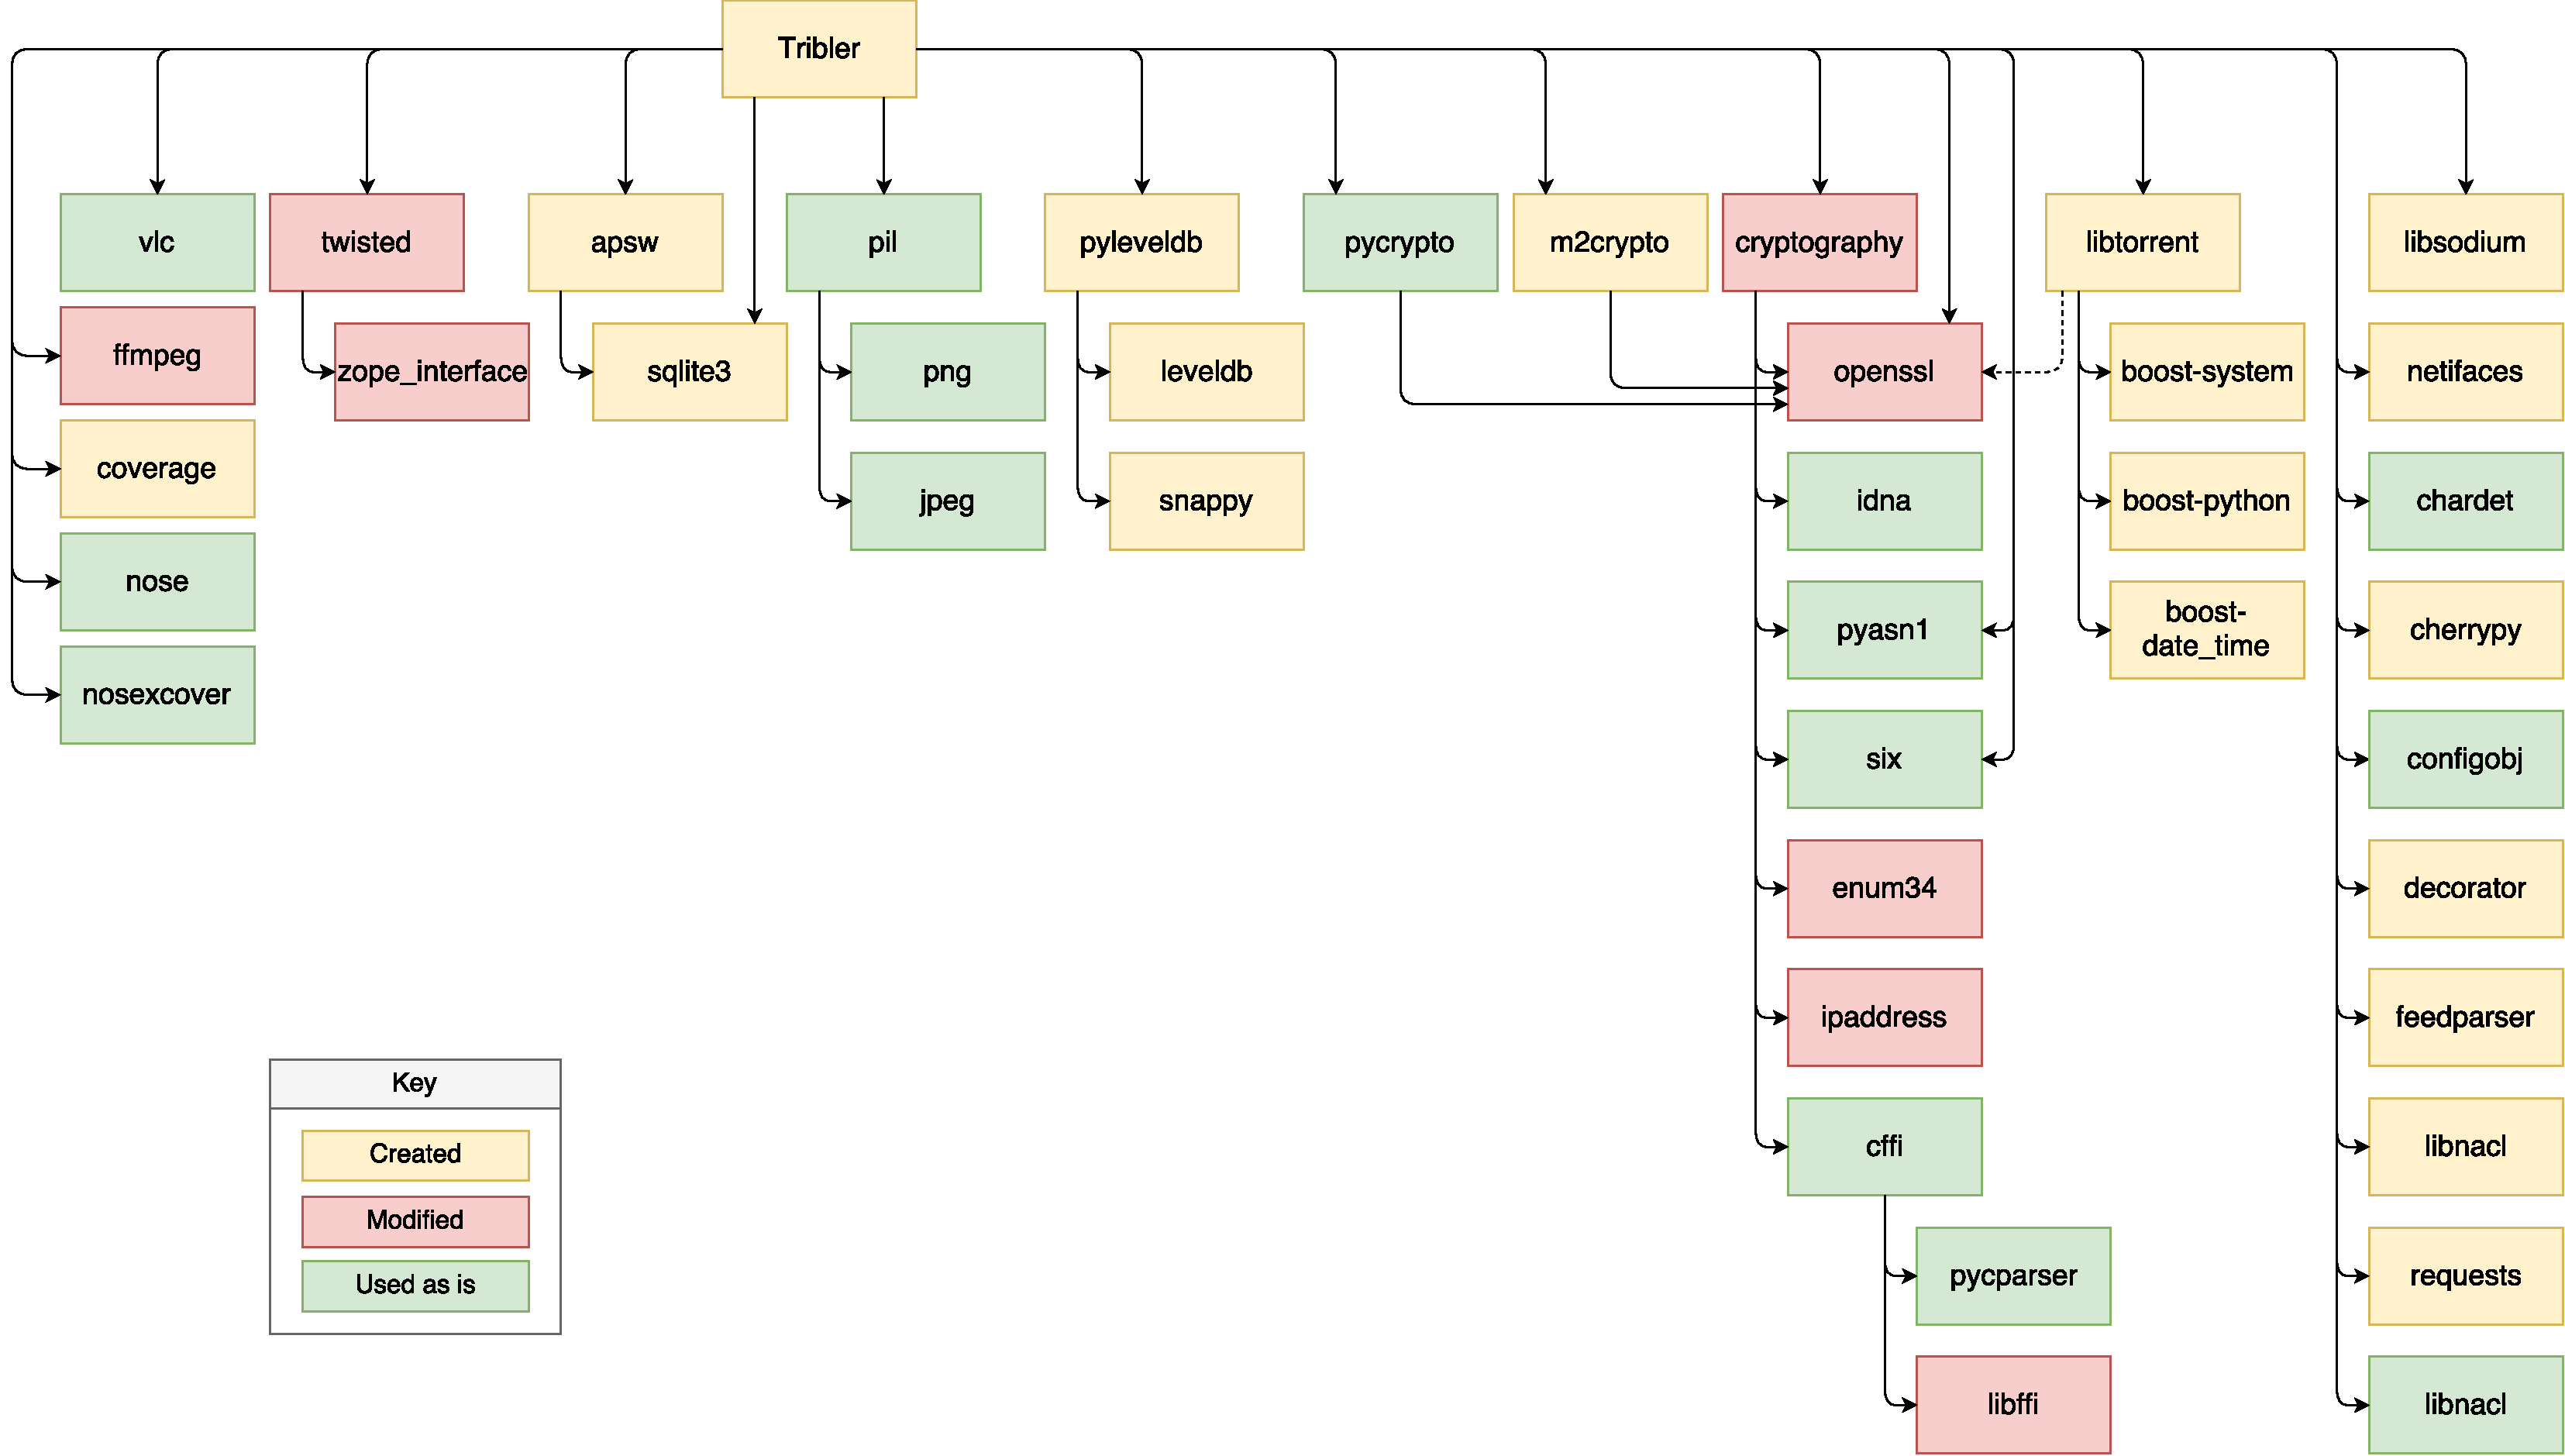
\includegraphics[width=\textwidth]{dependency_tree}
	\caption{Tribler dependencies in terms of Python-for-Android recipes}
	\label{fig:dependency_tree}
\end{figure}


The key performance indicators (KPI) will be \emph{scalability}, \emph{resource usage} of cpu, memory and power, and \emph{usability} in terms of latency.

\begin{figure}
	\centering
\begin{minipage}{.4\textwidth}
	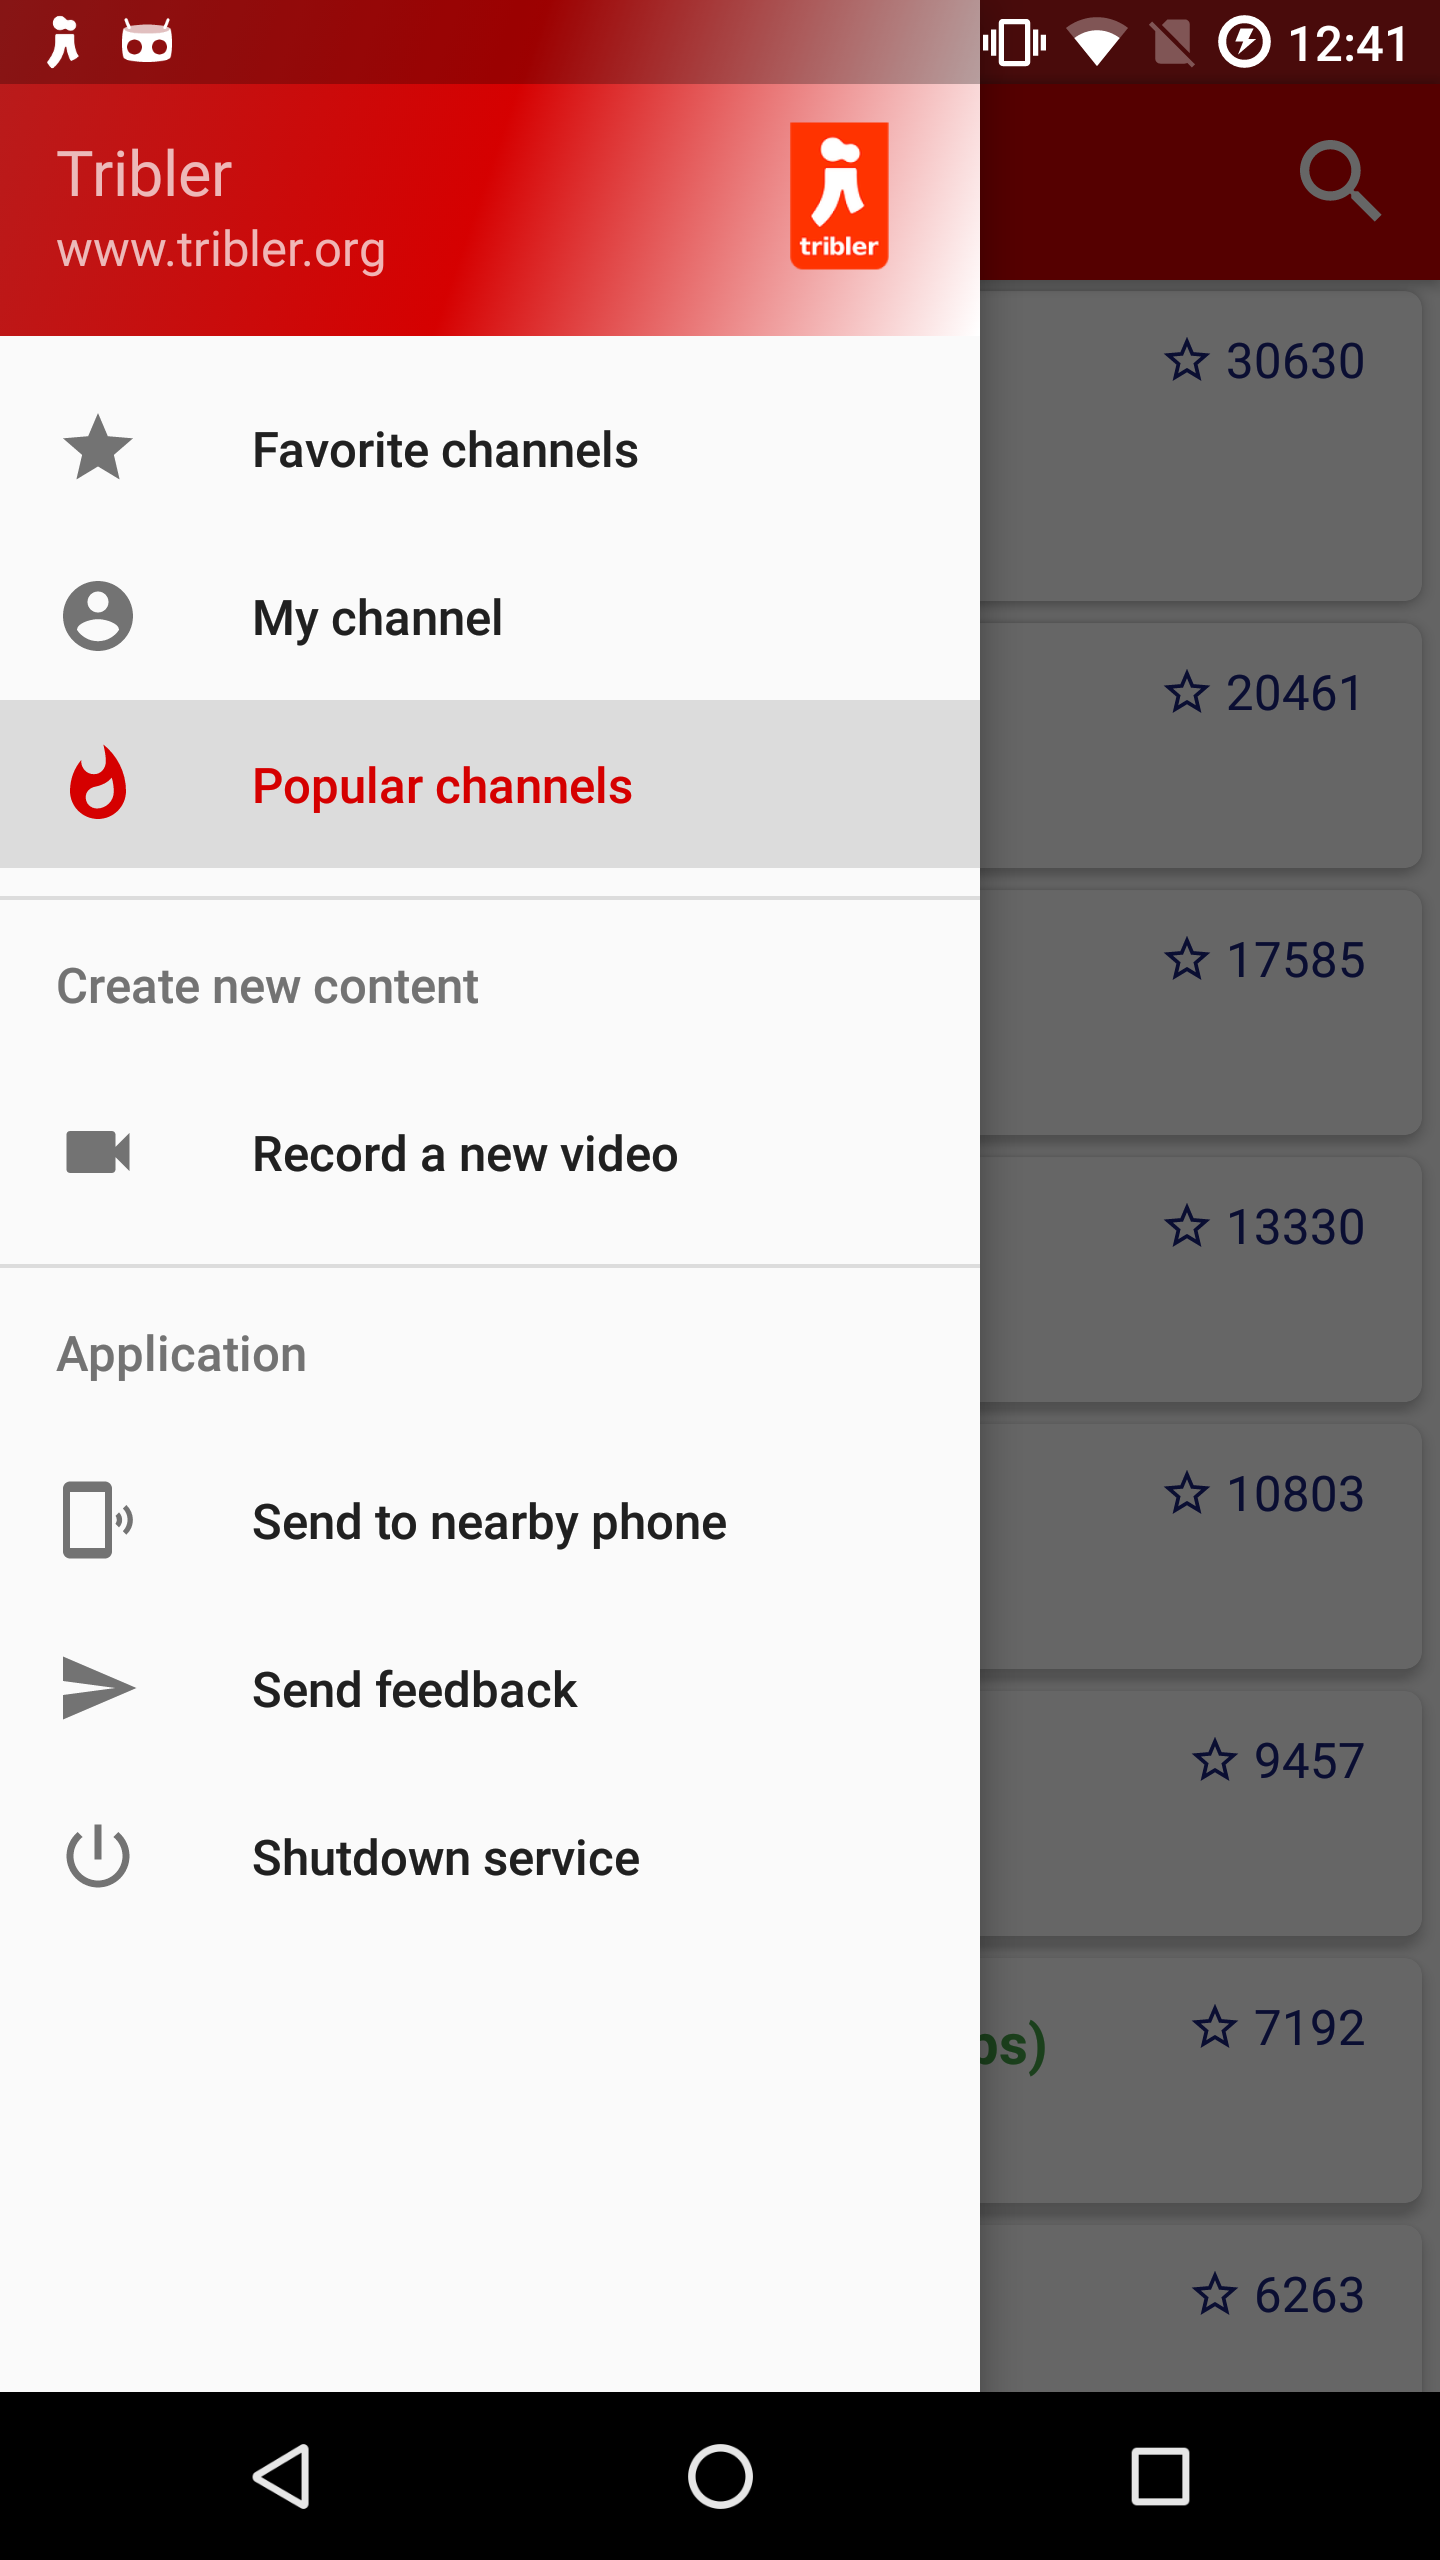
\includegraphics[width=\textwidth]{device-2016-08-28-menu-popular}
	\caption{Navigation menu of the Tribler app}
	\label{fig:menu-popular}
\end{minipage}
~
\begin{minipage}{.4\textwidth}
	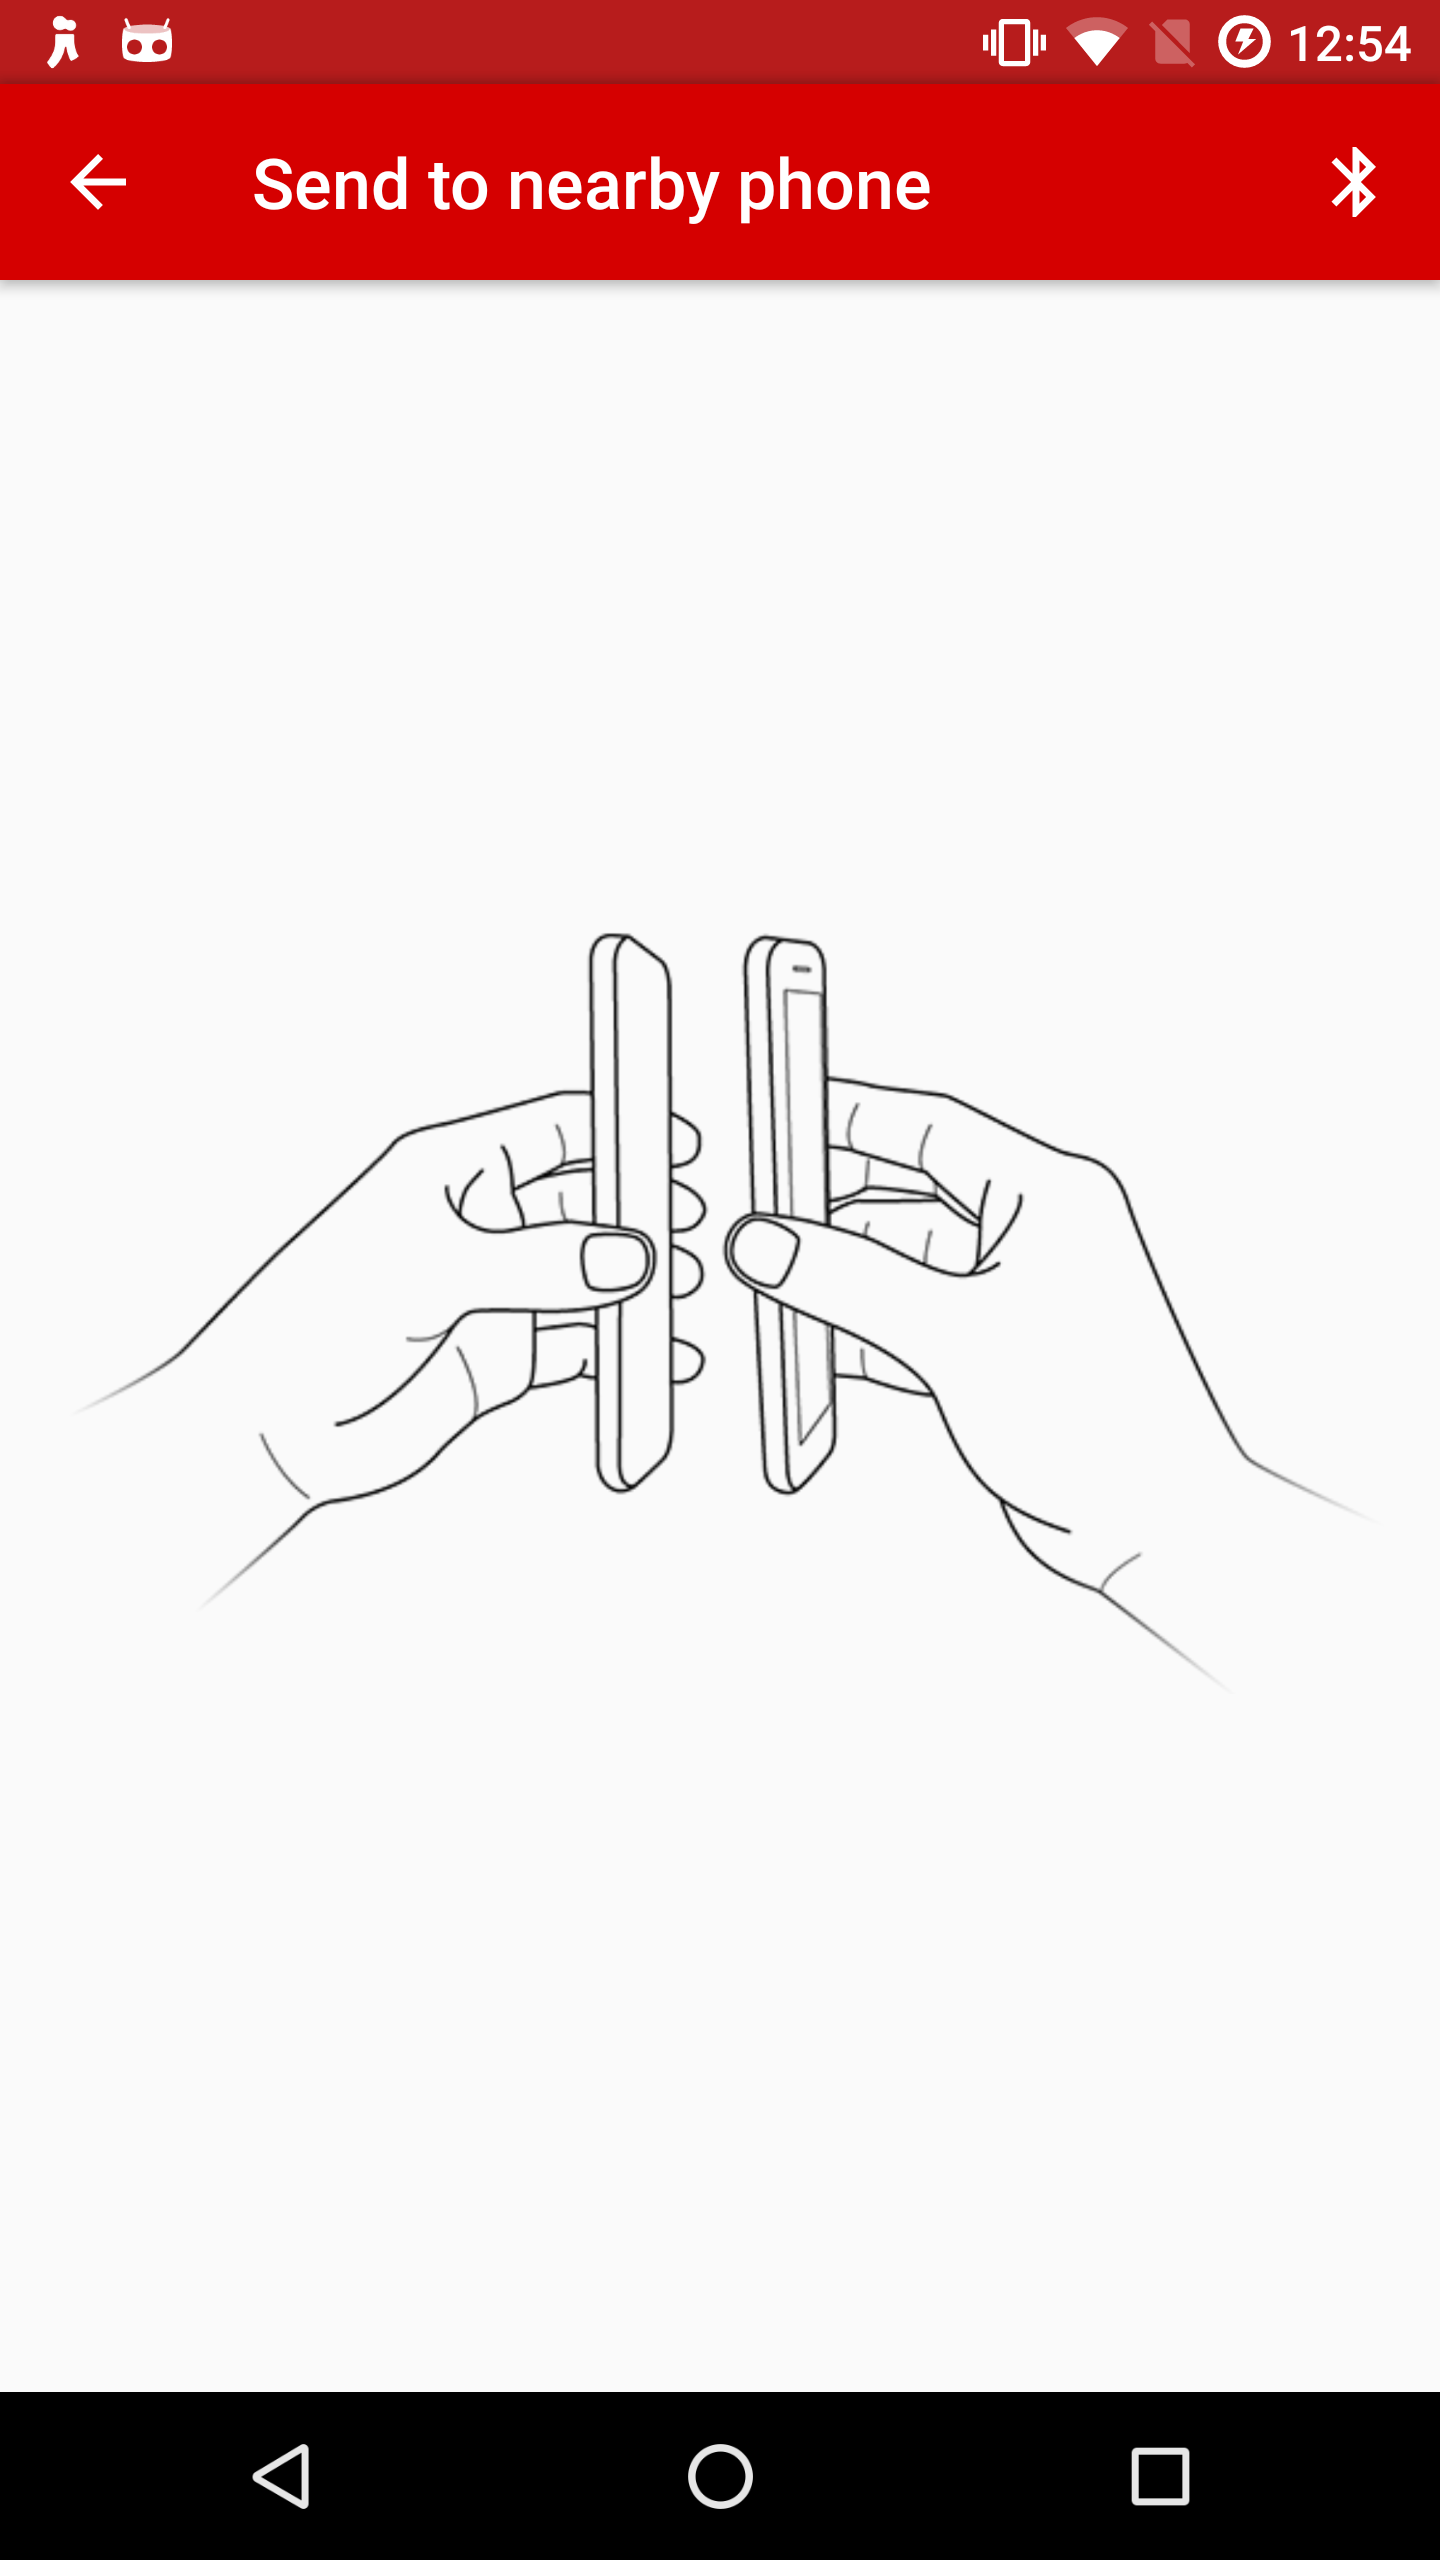
\includegraphics[width=\textwidth]{device-2016-08-28-beam}
	\caption{NFC+Bluetooth transfer of app or channel}
	\label{fig:beam}
\end{minipage}

\begin{minipage}{.4\textwidth}
	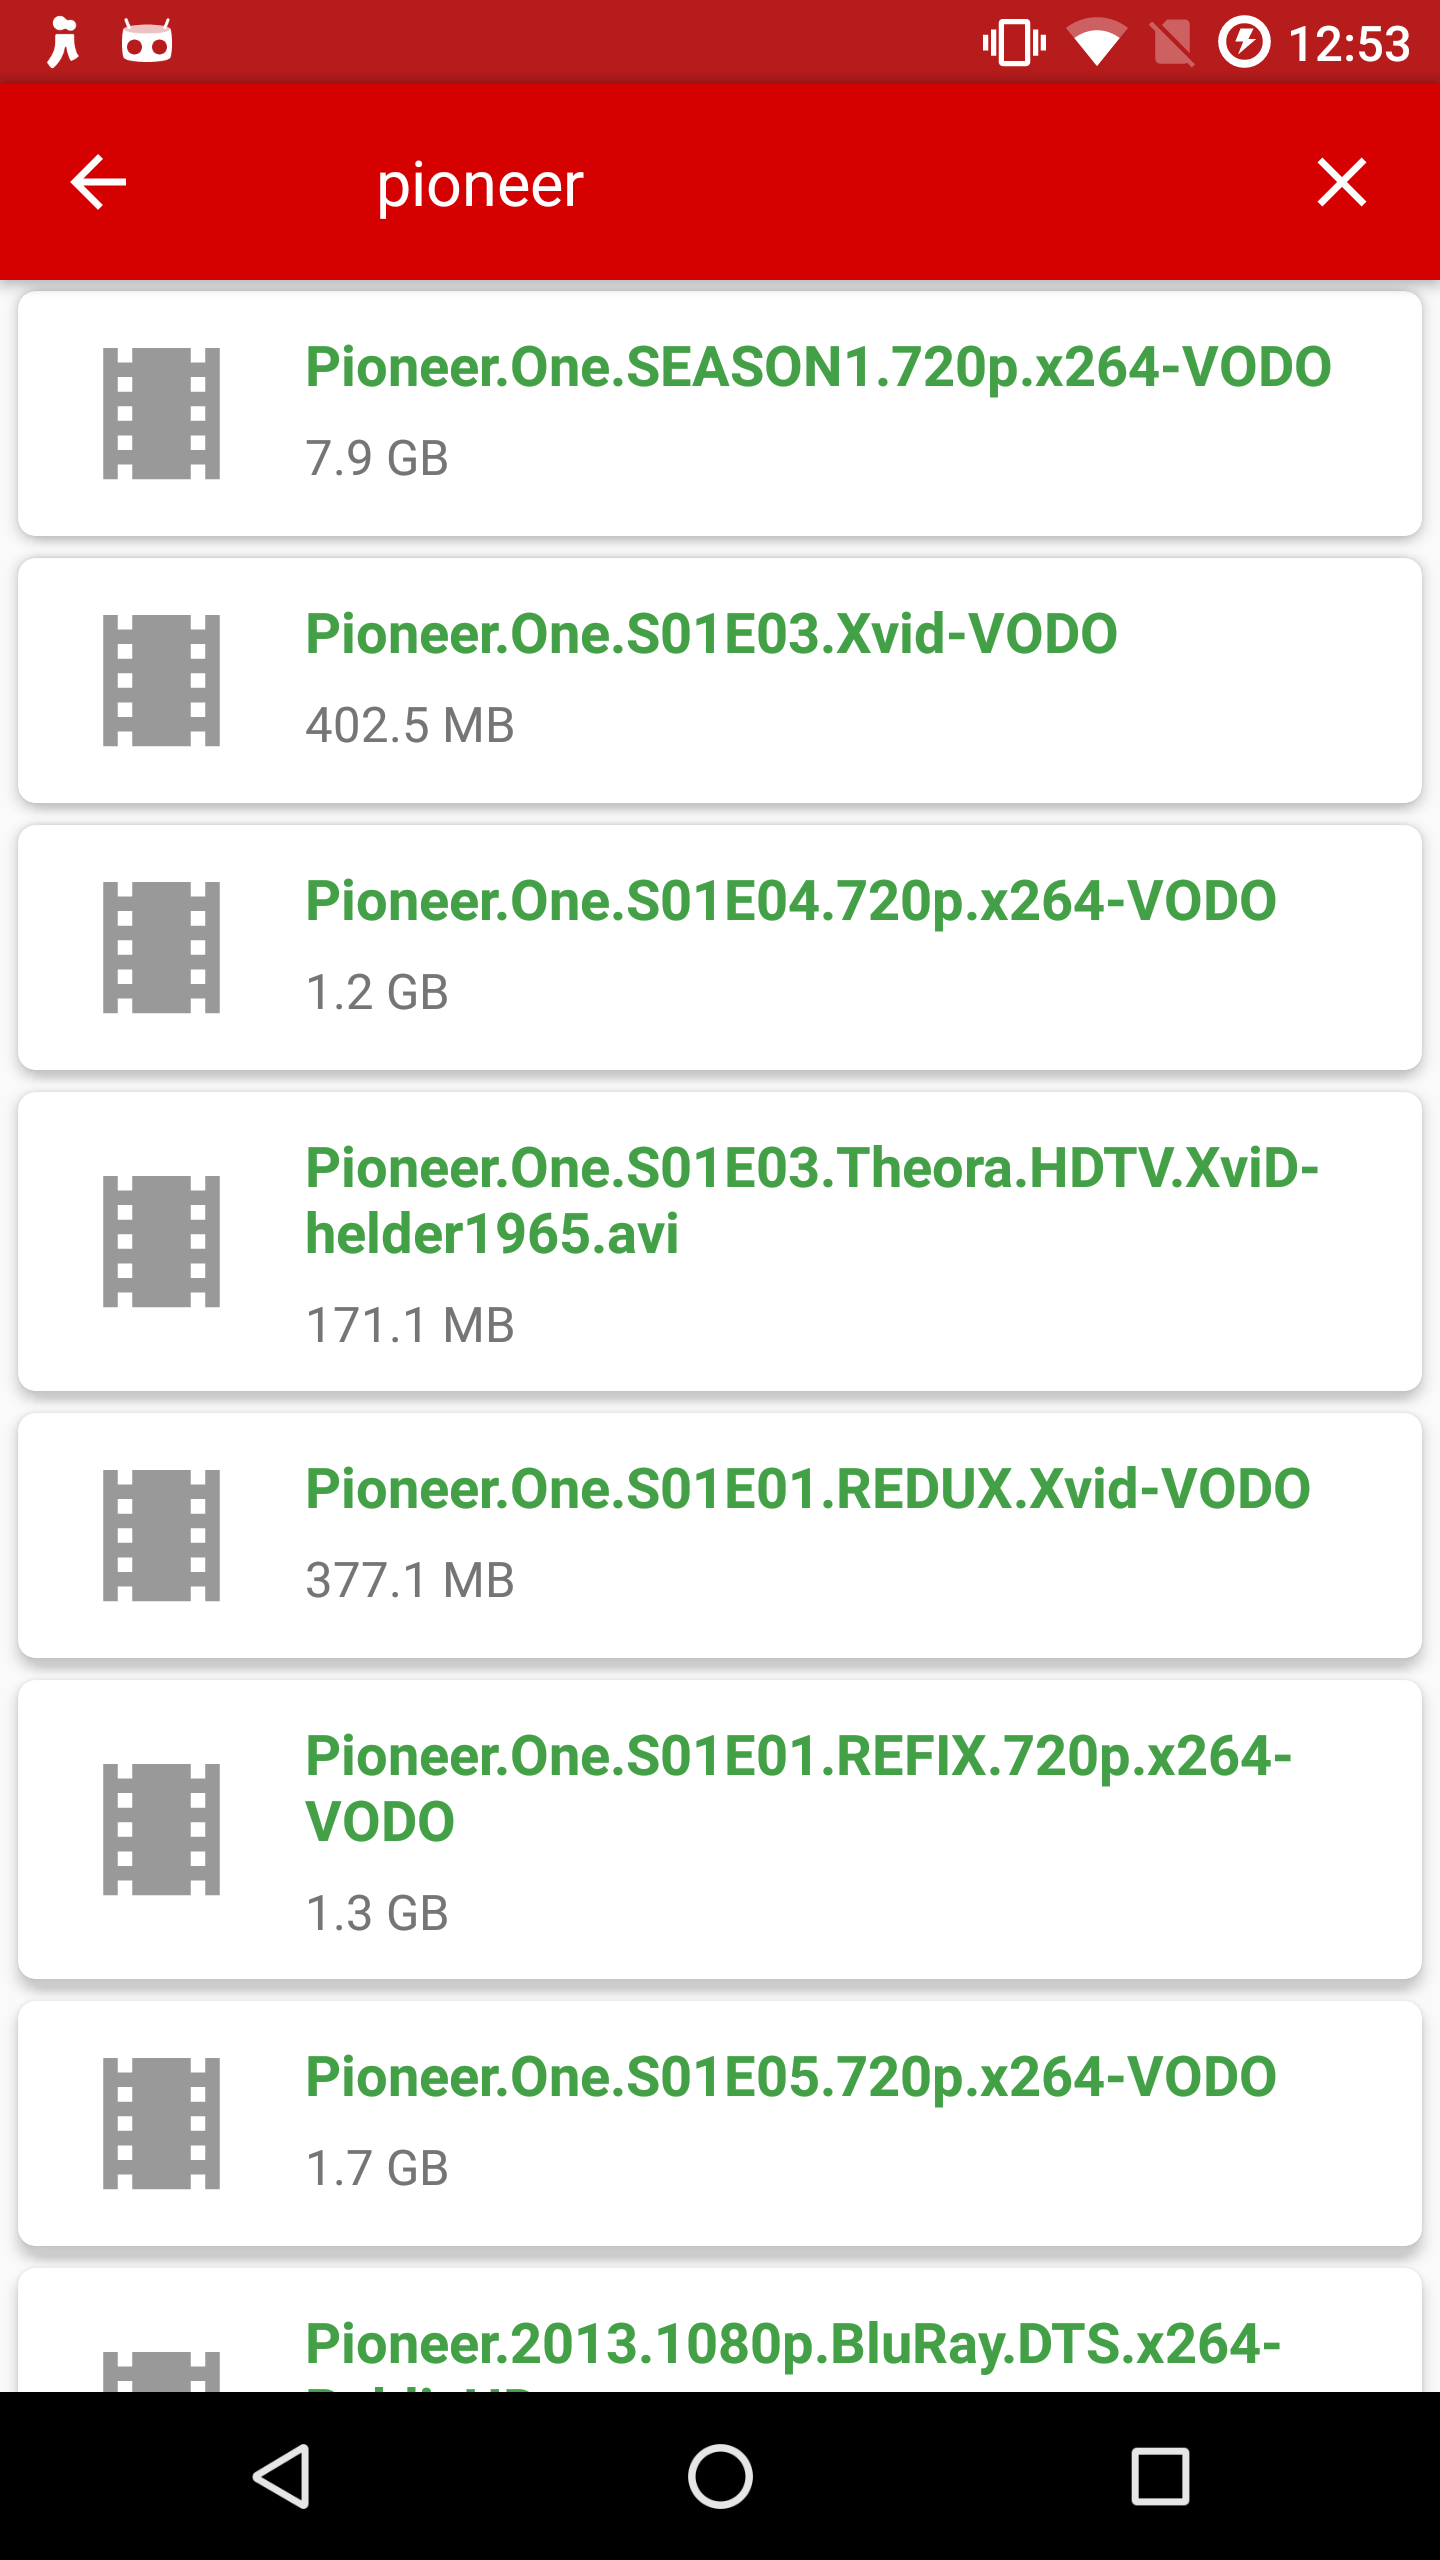
\includegraphics[width=\textwidth]{device-2016-08-28-search-pioneer}
	\caption{Search results showing video content}
	\label{fig:search-pioneer}
\end{minipage}
~
\begin{minipage}{.4\textwidth}
	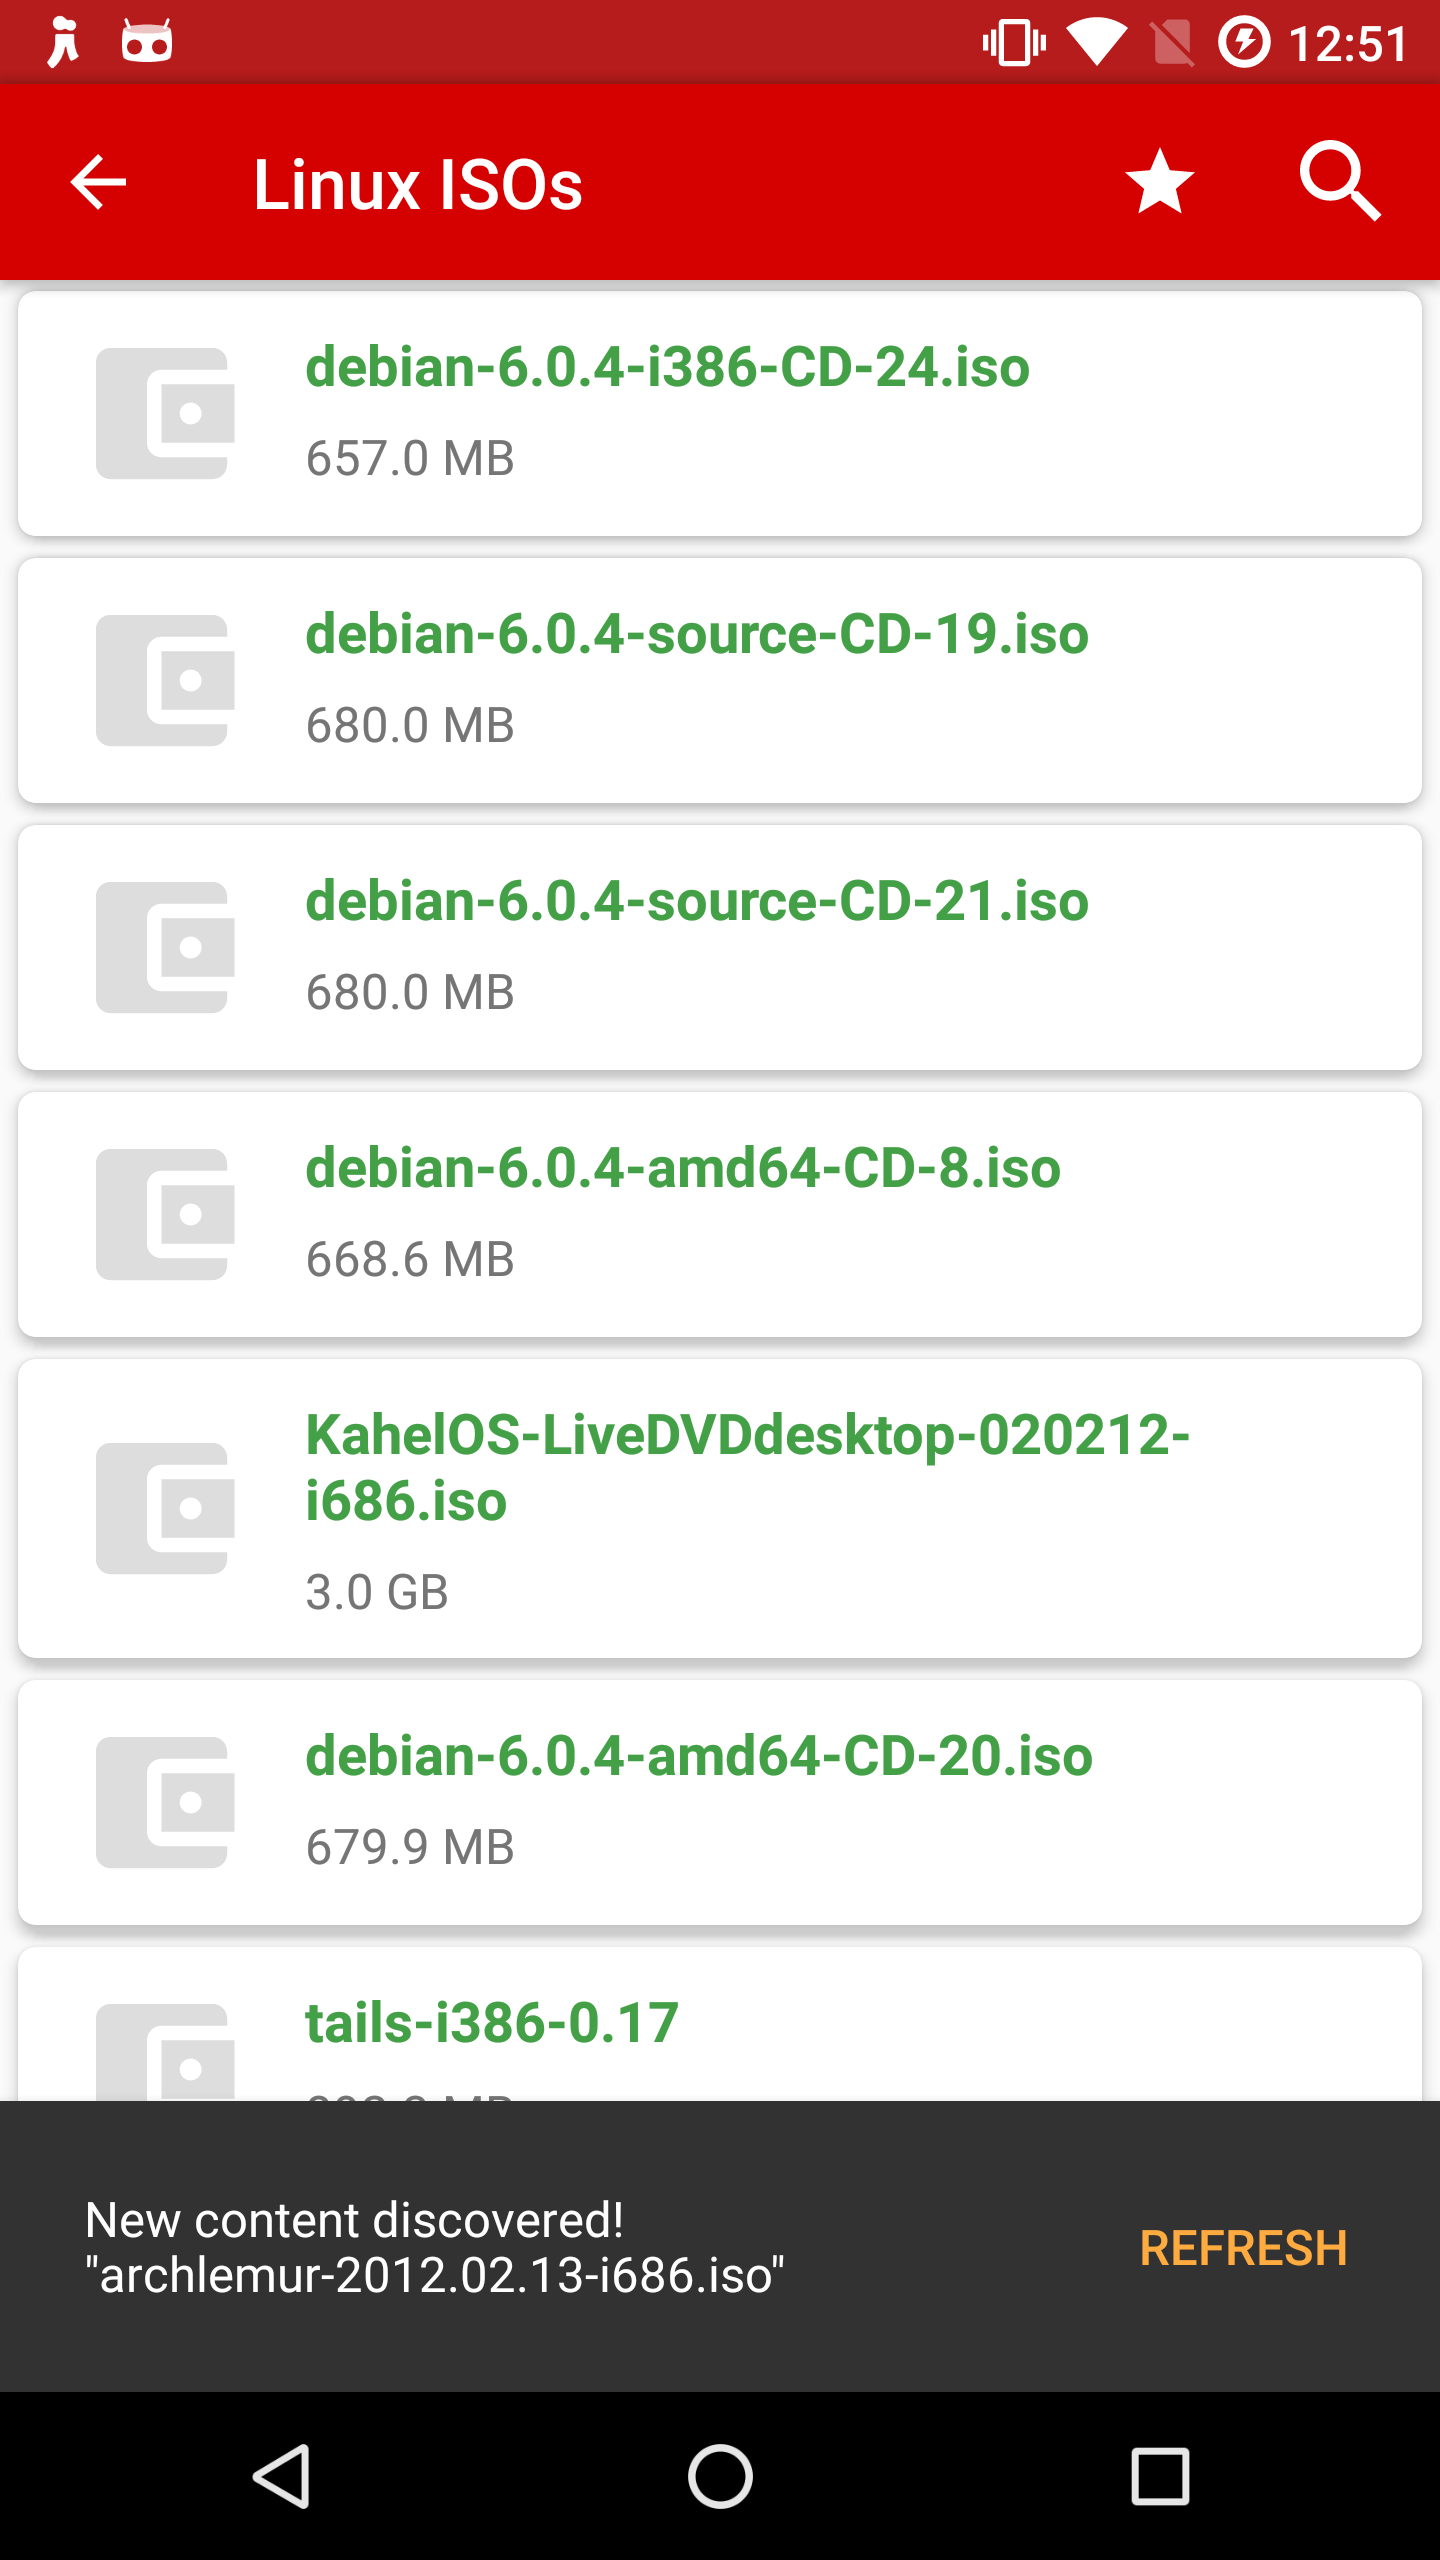
\includegraphics[width=\textwidth]{device-2016-08-28-channel-content-discovered}
	\caption{Channel with newly discovered content}
	\label{fig:channel-content-discovered}
\end{minipage}
\end{figure}